\documentclass[a4paper,12pt,twoside]{article}
\usepackage{braket}
\usepackage{graphicx}
\usepackage{amsmath}
\usepackage[english]{babel}
\usepackage[utf8]{inputenc}
\usepackage[colorlinks,bookmarks=false,citecolor={darkgreen},linkcolor=blue,urlcolor=blue]{hyperref}
\usepackage{color}
\usepackage[T1]{fontenc}
\usepackage{float}
\usepackage{url}
\usepackage{lscape}
\usepackage{tikz}
\usetikzlibrary{patterns,decorations.pathreplacing}
\usepackage[stable]{footmisc}
\usepackage{wrapfig}
\usepackage{textcomp}
\usepackage{changepage}
\usepackage{booktabs}
\usepackage{subfig}
\usepackage{amssymb}
\usepackage[section]{placeins}
\usepackage{mathabx}
\usepackage{comment} 
\usepackage{listings}
\usepackage{verbatim}
\usepackage{multicol}



\paperheight=297mm
\paperwidth=210mm

\setlength{\textheight}{235mm}
\setlength{\topmargin}{-1.2cm} 
\setlength{\textwidth}{15cm}
\setlength{\oddsidemargin}{0.56cm}
\setlength{\evensidemargin}{0.56cm}

\pagestyle{plain}

% def
\def \be {\begin{equation}}
\def \ee {\end{equation}}
\def \dd  {{\rm d}}
\def \bf {\textbf}
\def \bi {\begin{itemize}}
\def \ei {\end{itemize}}
\def \ib {\item[$\bullet$]}
\def \H {{\mathcal H}}
\def \grad{\nabla}
\def \( {\left(}
\def \) {\right)}
\def \order {{\cal O}}
\def \bc {\begin{comment}}
\def \ec {\end{comment}}
\def \defr {\textcolor{red}{Definition:}}
\def \db {\textcolor{blue}}
\def \remv {\textcolor{darkgreen}{Remarques:}}
\def \met {\textcolor{violet}{Méthode }}
\def \prop {\textcolor{darkgreen}{Propriétés:}}
\def \R {$\mathbb{R}$}
\def \D {$\mathbb{D}$}


\definecolor{ciel}{rgb}{0.04,0.52,0.78} % bleu ciel
\definecolor{darkgreen}{rgb}{0,0.5,0}% vert foncé
\definecolor{marron}{rgb}{0.32,0.19,0.19}%marron
\definecolor{violet}{rgb}{0.48,0.06,0.89}% violet
\definecolor{jaune}{rgb}{0.9,0.7,0.0} %jaune fonce


\def \swag{\textcolor{red}{S}\textcolor{ciel}{W}\textcolor{jaune}{A}\textcolor{darkgreen}{G}}



\newcommand{\mail}[1]{{\href{mailto:#1}{#1}}}
\newcommand{\ftplink}[1]{{\href{ftp://#1}{#1}}}
\newcommand{\e}{{\mathrm e}}
\renewcommand{\labelitemii}{$-$}


\newcommand{\thetaxy}{\theta_{X|Y }}
\newcommand{\thetayx}{\theta_{Y|X}}

\newcommand{\Nxy}{{N_{X|Y}}}
\newcommand{\Nyx}{{N_{Y|X}}}
\newcommand{\Nyy}{{N_{Y|Y}}}
\newcommand{\Nxx}{{N_{X|X}}}



\newcommand{\dxy}{{\delta_{X|Y}}}
\newcommand{\dyx}{{\delta_{Y|X}}}
\newcommand{\dyy}{{\delta_{Y|Y}}}
\newcommand{\dxx}{{\delta_{X|X}}}
\newcommand{\X}{\textcolor{red}{X}}
\newcommand{\Y}{\textcolor{blue}{Y}}

\title{Eigenfunction expansion of the refractory density} 

\author{No\'e Gallice \\ Professor: Wulfram Gerstner \hspace{0.5cm}  Supervisor: Tilo Schwalger\\ \small{ Laboratory of Computational Neuroscience, EPFL }
}

\date{January 8, 2018}


% ======= Le document commence ici ======

\begin{document}

\section{Laplace transform of the Survival function}

The Laplace transform of the ISI density $P_L(\lambda)$ at the (complex) arguments $\lambda_{n}$ must be unity. Where $\lambda_{n}$  are the eigenvalue of the refractory operator $\mathcal{L}$

\begin{equation}
\label{eq:conditionP}
1=\int_0^\infty e^{-\lambda_n \tau}P(\tau)\dd\tau=P_L(\lambda_n)\\
\end{equation}

We have a similar equation for the survival function for $n>0$

\begin{equation}
\label{eq:conditionS}
0=\int_0^\infty e^{-\lambda_n \tau}S(\tau)\dd\tau=S_L(\lambda_n)\\
\end{equation}

This can be derived using the fact that $P(\tau)=-\frac{\dd}{\dd \tau}S(\tau)$

\begin{eqnarray}
1=&\int_0^\infty e^{-\lambda_n \tau}P(\tau)\dd\tau\\
=&-\int_0^\infty e^{-\lambda_n \tau}\frac{\dd}{\dd \tau}S(\tau)\dd\tau \\
=& -e^{-\lambda_n \tau}S(\tau)|_0^\infty + \int_0^\infty -\lambda_ne^{-\lambda_n \tau}S(\tau)\dd\tau\\
=&1 -\lambda_n \int_0^\infty e^{-\lambda_n \tau}S(\tau)\dd\tau\\
\end{eqnarray}

Substracting $1$ on both side and diving by $ -\lambda_n$ we finally obtained Eq.\eqref{eq:conditionS}

We can also use the definition of the biothonormal basis $\langle\psi_i|\phi_j\rangle=\delta_{ij}$ and the fact that $\psi_0(\tau)=1$ thus for n>0:

\begin{eqnarray}
0=&\langle\psi_0|\phi_n\rangle\\
=&\int_0^\infty \phi_n(\tau) \dd\tau\\
=&\int_0^\infty \phi_n(0) e^{-\lambda_n \tau} S(\tau)\dd\tau\\
= &\phi_n(0) S_L(\lambda_n)
\end{eqnarray}


\section{Gamma process}

For a Gamma process the ISI density and it's  Laplace transform  are given by:

\begin{equation}
\label{eq:gamma}
P(\tau)=\frac{\beta^\gamma}{\Gamma(\gamma)}\tau^{\gamma-1}e^{-\beta\tau}
\end{equation}

\begin{equation}
\label{eq:gammaL}
P_L(\lambda)=\left(\frac{\beta}{\beta +\lambda}\right)^\gamma
\end{equation}

Using Eq.\eqref{eq:gammaL} and \eqref{eq:conditionP} we can find the spectrum  for this process

\begin{equation}
\label{eq:gammaeig}
\lambda_n=\beta\left(\exp\left(\frac{2\pi i}{\gamma}n\right)-1\right), \hspace{2.8cm}  n=0,..., \gamma-1
\end{equation}


Let's take an simple example, $\gamma=2$, according to Eq.\eqref{eq:gammaeig} there are 2eigenmodes with eigenvalue $\lambda_0=0$, $\lambda_1=-2\beta$, those eigenvalues satisfy$P_L(\lambda_n)=\left(\frac{\beta}{\beta +\lambda_n}\right)^2=1$, but if we try to compute explicitly the Laplace transform, a problem arises for $\lambda_1$:

\begin{eqnarray}
P_L(\lambda_1)=&\int_0^\infty e^{-\lambda_1 \tau}P(\tau)\dd\tau\\
=&\int_0^\infty e^{-\lambda_1 \tau}\beta^\gamma\tau e^{-\beta\tau}\dd\tau\\
=&\int_0^\infty\beta^\gamma\tau e^{+\beta\tau}\dd\tau
\end{eqnarray}

and this integral does not converge... \\


Writing explicitly the Laplace transform  for a general gamma process we have

\begin{equation}
\int_0^\infty e^{-\lambda_n \tau}P(\tau)\dd\tau
=\int_0^\infty e^{-(\lambda_n+\beta) \tau} \frac{\beta^\gamma}{\Gamma(\gamma)}\tau^{\gamma-1}e^{-\beta\tau}\dd\tau
\end{equation}

We see that the integral converge only if $\Re(\lambda_n)>-\beta$, this condition was already mention in Schwalger 2016.

The arising question are: \\
- are those eigenvalue meaningfull? \\
-if yes how to compute the coupling coefficient, for which similar diverging integrals are present.\\

To answer the first question let's look at the activity of population of neurons having an ISI density given by the gamma distribution. Too simplify the calculation the intial refractory density is given by a delta distribution i.e. $q(\tau,0)=\delta(\tau)$. In this case
$a_n(t)=exp(\lambda_n t )$ and the activity is given by:

\begin{equation}
\label{eq:A}
A(t)=\sum_n a_n(t)\phi_n(0)
\end{equation}

With 
\begin{equation}
\label{eq:phi0}
\phi_n(0)=\frac{1}{\gamma\beta^\gamma(\beta+\lambda_n)^{-(\gamma+1)}}
\end{equation}

The question is now:  is the sum  of Eq.\eqref{eq:A} running from $n=0 ...\gamma -1$, or just on the mode which satisfy the condition: $\Re(\lambda_n)>-\beta$. And in both case as we keep a finite number of mode do we recover an approximation or the exact solution of the population activity.

On Fig.\ref{fig:expan} we see that the complete expansion seems to be exact, thus the eigenvalue  which does not respect the condition $\Re(\lambda_n)>-\beta$, are useful to recover the exact solution.

Interestingly on fig.\ref{fig:q}, we see that with the complete expansion, we have a poor representation of the refractory density, if we compare it to the "true one" obtained by simulation. Nevertheless we see that at $\tau=0$, there is a match between both curves and thus we recover the correct activity $A(t)q(0,t)=A(t)$. This property was already observed in Schwalger 2016  for a poisson process.

This is not clear to me, how to explain this... it is like the refarctory density is not  in the subspace defined by the finite  eigenbasis. But the activity could be a projection on this subspace an thus is the correct one...


\begin{figure}[h!]
	\centering
	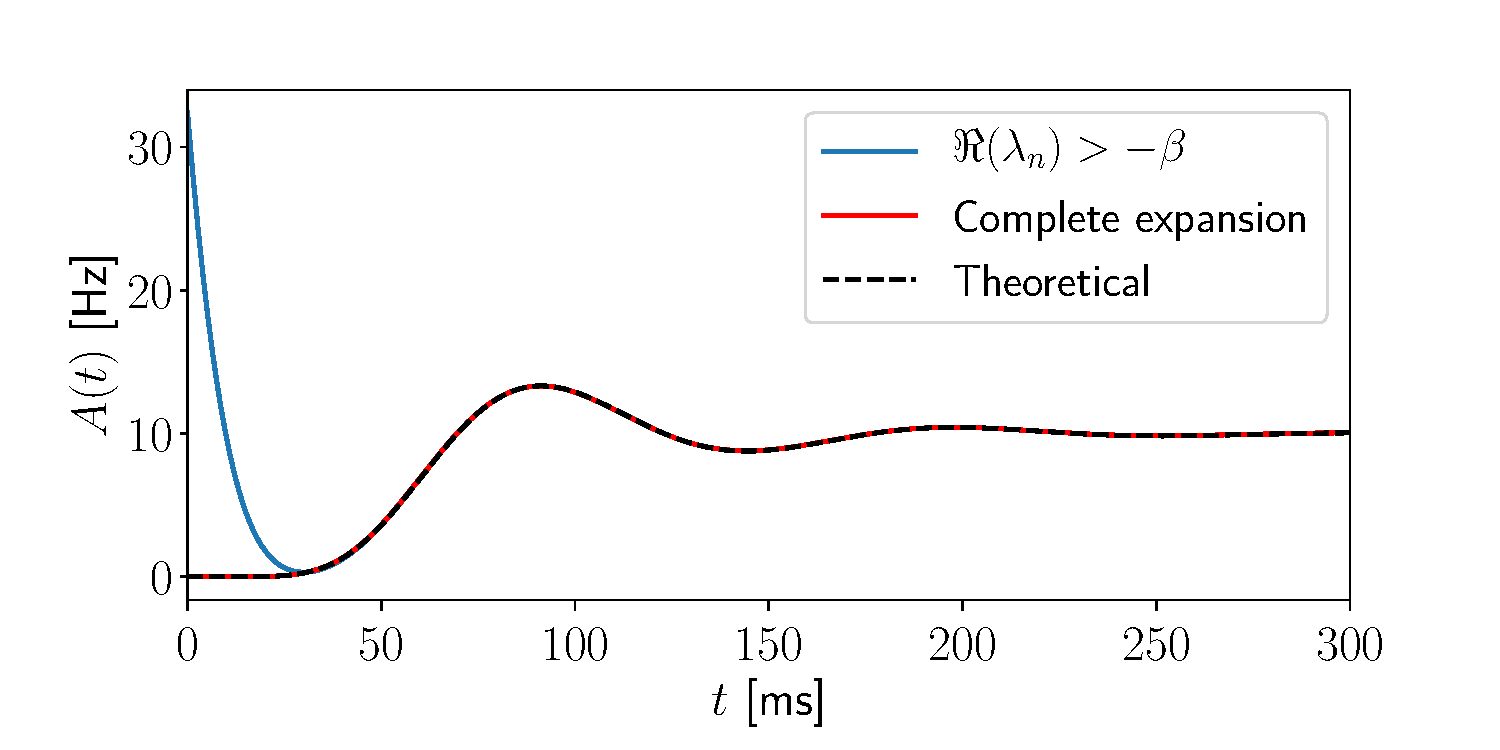
\includegraphics[width=0.8\linewidth]{expan.pdf}
	\caption{Activity $A(t)$ of a population of neurons having an ISI density given by the gamma distribution with $\beta=100$ Hz and $\gamma=10$ starting with a delta distribution $q(\tau,0)=\delta(\tau)$. }
	\label{fig:expan}
\end{figure}
	
	


\begin{figure}[h!]
	\centering
	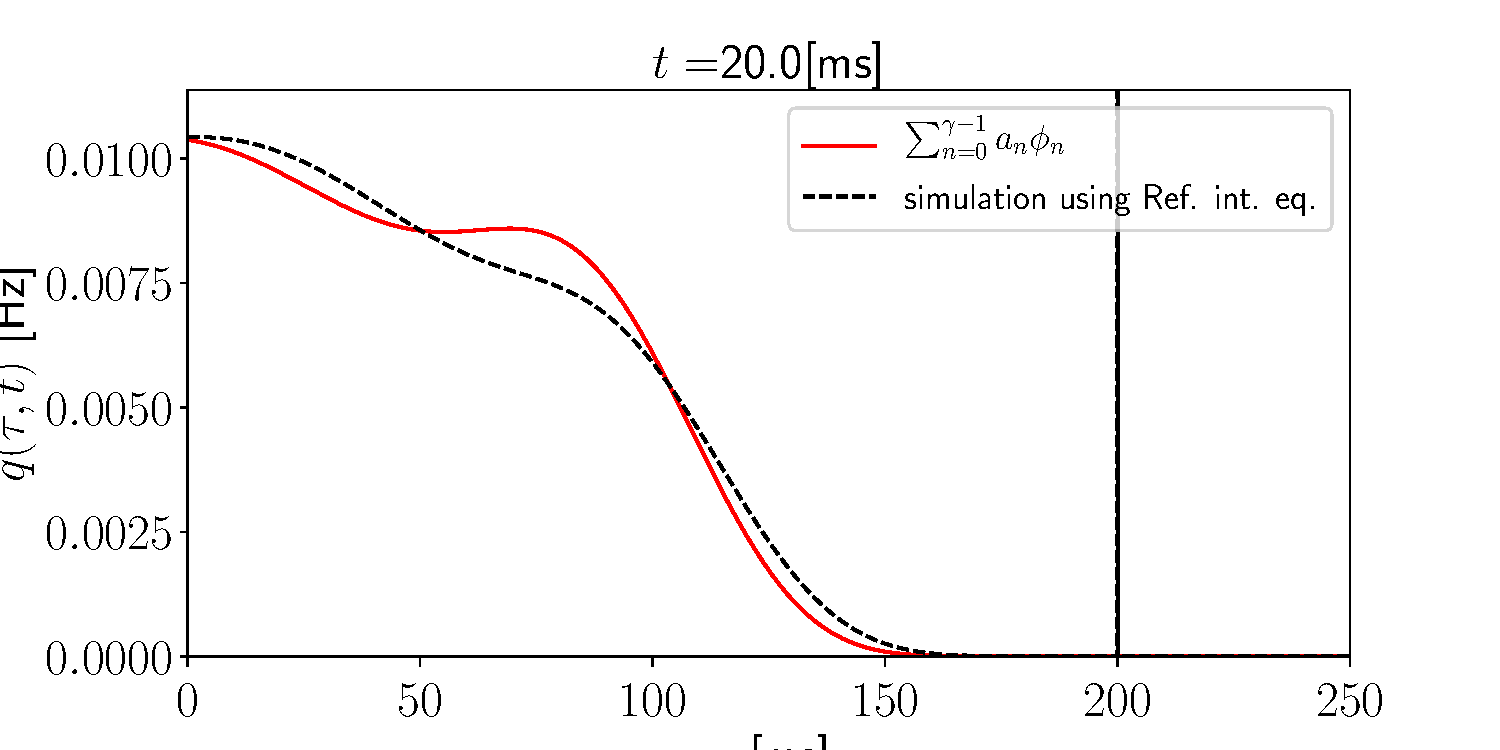
\includegraphics[width=0.8\linewidth]{q.pdf}
	\caption{Refractory density $q(\tau,t)$  at a certain time $t$ as a function of the age $tau$. The red line corresponds to the ones calculated using the expansion  with the 10 modes, the dash-black line correspond to the one obtained by numerical simulation using the integral formulation }
	\label{fig:q}
\end{figure}

\subsection{Toward an explanation for this particular initial condition}

We can describe the gamma process for $\gamma$ integer as a succession of $\gamma$ states with
rate $\beta$ between each state:

Thus with $P_i$ the neuron density  in sate $i$

\begin{equation}
\label{dotP}
\dot{P}_i=-\beta P_i+\beta P_{i-1} \hspace{1cm} i=2,...\gamma
\end{equation}

and 

\begin{equation}
\label{dotP1}
\dot{P}_1=-\beta P_1+\beta P_{\gamma}
\end{equation}

We have 
\begin{equation}
\sum_{i=1}^{\gamma}P_i=1
\end{equation}
 and 
 \begin{equation}
 \label{eq:AP}
A(t)=\beta P_\gamma
 \end{equation}
 
 Lets prove that  if $P_1(0)=1$ (equivalent to have $q(\tau,0)=\delta(0)$) then 

 
  \begin{equation}
   \label{eq:Asum}
 A(t)=\sum_{n=0}\frac{\beta}{\gamma}\pi_n exp(\beta(\pi_n-1)t)
  \end{equation}

We just rewrite Eq \eqref{eq:A}, using Eq.\eqref{eq:phi0} and Eq.\eqref{eq:gammaeig} and  introducing the notation $\pi_n= \exp\left(\frac{2\pi i}{\gamma}n\right)$

From Eq.\eqref{eq:AP} and Eq.\eqref{eq:Asum}:
 \begin{equation}
  P_\gamma=\sum_{n=0}\frac{1}{\gamma}\pi_n exp(\beta(\pi_n-1)t)
 \end{equation}
 
 and deriving the previous we have
 
 \begin{equation}
 \dot{P}_\gamma=\sum_{n=0}\frac{\beta(\pi_n^2-\pi_n)}{\gamma}exp(\beta(\pi_n-1)t)
 \end{equation}
 
 and using Eq.\eqref{dotP} we deduce that
 
 \begin{equation}
  P_{\gamma-1}=\sum_{n=0}\frac{1}{\gamma}\pi_n^2 exp(\beta(\pi_n-1)t)
 \end{equation}
 
 by recurrence we can find
 
 \begin{equation}
 \label{eq:Pi}
P_{i}=\sum_{n=0}\frac{1}{\gamma}\pi_n^{\gamma+1-i} exp(\beta(\pi_n-1)t)=P_{i}=\sum_{n=0}\frac{1}{\gamma}\pi_n^{1-i} exp(\beta(\pi_n-1)t)
\end{equation}

and we can verify that Eq.\eqref{dotP1} is satisfied.

Also using the fact that 
 \begin{equation}
\sum_{n=0}\frac{1}{\gamma}\pi_n^{1-i} =0 \hspace{1cm} for \hspace{0.5cm} i=2,....,\gamma
\end{equation}

We see that $P_1(0)=1$ and $P_i(0)=0$
\subsection{Matrix form}
We can write the previous system of first order differential equations Eq.\eqref{dotP} introducing the squared Matrix $A$ of size $\gamma$:  $\dot{ \textbf{P}}=A\textbf{P}$

 \begin{equation}
\dot{ \textbf{P}}=\beta
\begin{pmatrix}
-1&           & &1 \\
  1&\ddots& &   \\
    &\ddots&\ddots &   \\
      & &1& -1  
\end{pmatrix}
\textbf{P}
 \end{equation}
 
 and the solution of this system is then:
 $\textbf{P}(t)=e^{At}\textbf{P}(0)$
 
 the eigenvalues of Matrix $A$ are the same as Eq.\eqref{eq:gammaeig}
 
 \begin{equation}
 \label{eq:gammaeig1}
 \lambda_n=\beta\left(\exp\left(\frac{2\pi i}{\gamma}n\right)-1\right), \hspace{2.8cm}  n=0,..., \gamma-1
 \end{equation}
 
 It's not always simple to compute the term $e^{At}$ but for $\textbf{P}(0)=
 \begin{pmatrix}
 1 \\
0  \\
 \vdots   \\
0
 \end{pmatrix}$

we know the solution thus we know the elements of the first column of the matrix  $e^{At}$ , they are given by equation Eq.\eqref{eq:Pi}, and using the symmetry of the system, we know that the matrix $e^{At}$  has the form:

 \begin{equation}
e^{At}=
\begin{pmatrix}
a_1 & a_\gamma& \dots&a_2\\
a_2&  a_1 & \dots & a_3\\
\vdots& \vdots&\ddots  &\vdots  \\
a_\gamma & a_{\gamma-1}&\dots&a_1
\end{pmatrix}
\end{equation}

So we know every elements of the matrix $e^{At}$, note that here $\beta$ is fixed.
The question now is how to translate a general age initial distribution $q(\tau,0)$ in a vector $\textbf{P}(0)$

Now if $\beta$ is time dependent we just have to change,  $\textbf{P}(t)=e^{At}\textbf{P}(0)$ for
\begin{equation}
 \textbf{P}(t)=e^{A\int_{0}^{t}\beta(s)\dd s}\textbf{P}(0)
\end{equation}

and replace in Eq.\eqref{eq:Pi}, the factor $\beta t$ by $\int_{0}^{t}\beta(s)\dd s$

 
 

\section{Gamma process with $\gamma$ an Integer}
ISI density:
\begin{equation}
\label{eq:P}
P(\tau)=\frac{\beta^\gamma}{\Gamma(\gamma)}\tau^{\gamma-1}e^{-\beta\tau}=\frac{\beta^\gamma}{(\gamma-1)!}\tau^{\gamma-1}e^{-\beta\tau}
\end{equation}

Survival:
\begin{eqnarray}
\label{eq:S}
S(\tau)=&\frac{\Gamma(\gamma,\beta\tau)}{\Gamma(\gamma)}=\frac{1}{\Gamma(\gamma)}\int_{\beta\tau}^{\infty}x^{\gamma-1}e^{-x}\dd x\\
=&e^{-\beta \tau}[\sum_{k=0}^{\gamma-1}\frac{(\beta\tau)^k}{k!}]
\end{eqnarray}

Hazard rate:
\begin{eqnarray}
\label{eq:RHO}
\rho(\tau)&=&\frac{P(\tau)}{S(\tau)}\\
&=&\frac{\beta^\gamma\tau^{\gamma-1}}{(\gamma-1)![\sum_{k=0}^{\gamma-1}\frac{(\beta\tau)^k}{k!}]}
\end{eqnarray}

Spectrum:
\begin{equation}
\label{eq:eig}
\lambda_n=\beta\left(\exp\left(\frac{2\pi i}{\gamma}n\right)-1\right), \hspace{1cm}  n= -\gamma/2-1,...,0,...,+ \gamma/2-1  
\end{equation}

introducing the notation $\pi_n= \exp\left(\frac{2\pi i}{\gamma}n\right)$

\begin{equation}
\label{eq:eig1}
\lambda_n=\beta\left(\pi_n-1\right)
\end{equation}


Normalisation:
\begin{eqnarray}
\phi_n(0)&=&\frac{(\beta+\lambda_n)^\gamma+1}{\gamma\beta^\gamma}\\
&=&\frac{\beta}{\gamma}\pi_n
\end{eqnarray}

Where we use the fact that $\pi_n^\gamma=1$

Eigenfunctions:
\begin{align}
\label{eq:phin}
\phi_n(\tau)&=\phi_n(0)e^{-\lambda_n\tau}S(\tau)\\
&=\frac{\beta}{\gamma}\pi_ne^{-\beta\pi_n\tau}[\sum_{k=0}^{\gamma-1}\frac{(\beta\tau)^k}{k!}]
\end{align}

\begin{align}
\label{eq:psin}
\psi_n(\tau)&=e^{\lambda_n\tau}\big[1-\int^\tau_0 \dd x P(x) e^{-\lambda_nx}\big]\frac{1}{S(\tau)}\\
&=\frac{e^{\beta\pi_n\tau}}{\sum_{k=0}^{\gamma-1}\frac{(\beta\tau)^k}{k!}}[1-\int_0^\tau \dd x \frac{\beta^\gamma}{(\gamma-1)!}\tau^{\gamma-1}e^{-\beta\pi_n\tau}]\\
&=\frac{e^{\beta\pi_n\tau}}{\sum_{k=0}^{\gamma-1}\frac{(\beta\tau)^k}{k!}}[1-\pi_n^{-\gamma}(1-e^{-\beta\pi_n\tau}[\sum_{k=0}^{\gamma-1}\frac{(\beta\pi_n\tau)^k}{k!}])]\\
&=\frac{\sum_{k=0}^{\gamma-1}\frac{(\beta\pi_n\tau)^k}{k!}}{\sum_{k=0}^{\gamma-1}\frac{(\beta\tau)^k}{k!}}
\end{align}


Coupling coefficient:
\begin{equation}
\label{eq:couplingcoef}
C_{nm}=\langle\partial_h\psi_n|\phi_m \rangle 
\end{equation}

Let's say that only $\beta$ depends on h 

\begin{equation}
\label{eq:couplingcoefdb}
C_{nm}=\frac{\partial \beta}{\partial h}\langle\partial_\beta\psi_n|\phi_m \rangle 
\end{equation}

Lets compute $\partial_\beta\psi_n$:

\begin{align}
\label{eq:psindb}
\frac{\partial\psi_n}{\partial \beta}&=\frac{\sum_{k=1}^{\gamma-1}\frac{\beta^{k-1}(\pi_n\tau)^k}{(k-1)!}}{\sum_{k=0}^{\gamma-1}\frac{(\beta\tau)^k}{k!}}-\frac{\sum_{k=0}^{\gamma-1}\frac{(\beta\pi_n\tau)^k}{k!}}{[\sum_{k=0}^{\gamma-1}\frac{(\beta\tau)^k}{k!}]^2}[\sum_{k=1}^{\gamma-1}\frac{\beta^{k-1}(\tau)^k}{(k-1)!}]\\
&=\frac{\sum_{k=0}^{\gamma-2}\frac{\beta^{k}(\pi_n\tau)^{k+1}}{k!}}{\sum_{k=0}^{\gamma-1}\frac{(\beta\tau)^k}{k!}}-\frac{\sum_{k=0}^{\gamma-1}\frac{(\beta\pi_n)^k\tau^{k+1}}{k!}}{[\sum_{k=0}^{\gamma-1}\frac{(\beta\tau)^k}{k!}]}+\frac{\frac{\beta^{\gamma-1}\tau^\gamma}{(\gamma-1)!}\sum_{k=0}^{\gamma-1}\frac{(\beta\pi_n\tau)^k}{k!}}{[\sum_{k=0}^{\gamma-1}\frac{(\beta\tau)^k}{k!}]^2}\\
&=f_1(\tau)-f_2(\tau)+f_3(\tau)
\end{align}

Lets compute separatly $\langle f_i|\phi_m \rangle$  for those three terms

\begin{equation}
\label{eq:integrale}
\int_0^\infty x^a e^{-bx}=\frac{a!}{b^{a+1}}
\end{equation}


\begin{align}
\langle f_1|\phi_m \rangle&=\sum_{k=0}^{\gamma-2}\frac{\beta^{k+1}}{\gamma}\frac{\pi_n^{k+1}\pi_m}{k!}\int^\infty_0\tau^{k+1}e^{-\beta\pi_m\tau}\\
&=\frac{1}{\beta\gamma}\sum_{k=0}^{\gamma-2}(\frac{\pi_n}{\pi_m})^{k+1}(k+1)\\
&=\frac{1}{\beta\gamma}\sum_{k=1}^{\gamma-1}k\pi_{n-m}^{k}
\end{align}

\begin{align}
\langle f_2|\phi_m \rangle&=\sum_{k=0}^{\gamma-1}\frac{\beta^{k+1}}{\gamma}\frac{\pi_n^{k}\pi_m}{k!}\int^\infty_0\tau^{k+1}e^{-\beta\pi_m\tau}\\
&=\frac{1}{\beta\gamma\pi_n}\sum_{k=1}^{\gamma}k\pi_{n-m}^{k}\\
&=\frac{1}{\beta\pi_n}+\frac{1}{\beta\gamma\pi_n}\sum_{k=1}^{\gamma-1}k\pi_{n-m}^{k}
\end{align}


\begin{align}
\langle f_3|\phi_m \rangle&=\int_0^\infty\frac{e^{-\beta\pi_m\tau}\pi_m\frac{\beta^{\gamma}\tau^\gamma}{\gamma!}\sum_{k=0}^{\gamma-1}\frac{(\beta\pi_n\tau)^k}{k!}}{\sum_{k=0}^{\gamma-1}\frac{(\beta\tau)^k}{k!}}\dd \tau
\end{align}

I don't know why but it turns out that 
$\langle f_3|\phi_m \rangle\simeq \frac{1}{\beta}$

Thus 

\begin{equation}
\langle\partial_\beta\psi_n|\phi_m \rangle =\frac{1}{\beta}(1-\frac{1}{\pi_{n}})[1+\frac{1}{\gamma}\sum_{k=1}^{\gamma-1}k\pi_{n-m}^{k}]
\end{equation}

\begin{equation}
\label{eq:cnm}
C_{nm}=\frac{\partial \beta}{\partial h}\frac{1}{\beta}(1-\frac{1}{\pi_{n}})[\frac{1}{\gamma}\sum_{k=1}^{\gamma}k\pi_{n-m}^{k}]
\end{equation}

Rate:
\begin{equation}
\beta(h)=\beta_0 exp(\kappa(h-h_0))
\end{equation}

\begin{equation}
\label{eq:cnm3}
C_{nm}=\kappa(1-\frac{1}{\pi_{n}})[\frac{1}{\gamma}\sum_{k=1}^{\gamma}k\pi_{n-m}^{k}]
\end{equation}

\begin{equation}
\label{eq:c10}
C_{10}=1
\end{equation}

\begin{equation}
\label{eq:c11}
C_{11}=(\gamma +1 )[\sin^2\frac{\pi}{\gamma}+i\sin\frac{\pi}{\gamma}\cos\frac{\pi}{\gamma}]
\end{equation}

\begin{equation}
\label{eq:c11}
C_{1-1}=\frac{1}{2}[1+i\tan\frac{\pi}{\gamma}]
\end{equation}




\end{document} %%%% THE END %%%%